\documentclass[letterpaper]{article}
\def\aaaianonymous{true}
\usepackage[submission]{aaai2026}
\usepackage{times}
\usepackage{helvet}
\usepackage{courier}
\usepackage[hyphens]{url}
\usepackage{graphicx}
\urlstyle{rm}
\def\UrlFont{\rm}
\usepackage{natbib}
\usepackage{caption}
\frenchspacing
\setlength{\pdfpagewidth}{8.5in}
\setlength{\pdfpageheight}{11in}
\usepackage{amsmath}
\usepackage{booktabs}
\usepackage{array}
\usepackage{multirow}
\usepackage{xcolor}
\usepackage{pgfplots}
\pgfplotsset{compat=1.18}
\usepackage{tikz}
\usetikzlibrary{arrows.meta,positioning,fit,calc,shapes.geometric}
\usepackage{xspace}
\usepackage{algorithm}
\usepackage{algorithmic}

\newcommand{\method}{BudgetFlow\xspace}
\newcommand{\trv}{TRV\xspace}
\newcommand{\taskvalue}{Task Value\xspace}
\newcommand{\tokencost}{Estimated Token Cost\xspace}
\newcommand{\modelfit}{Model Fit\xspace}
\newcommand{\sharedbudget}{Shared Budget\xspace}
\newcommand{\verifier}{Verifier\xspace}
\newcommand{\pos}[1]{\textcolor{red}{\textbf{#1}}}
\newcommand{\ctrl}[1]{\textcolor{blue}{\textbf{#1}}}
\definecolor{bfred}{HTML}{C62828}
\definecolor{bfblue}{HTML}{1565C0}
\definecolor{bfteal}{HTML}{00897B}
\definecolor{bforange}{HTML}{EF6C00}
\definecolor{bfgray}{HTML}{6D6D6D}

\pdfinfo{/TemplateVersion (2026.1)}

\title{BudgetFlow: Value-Aware Budget Governance for Agent Tasks}
\author{
    Anonymous Author(s)\\
    Affiliation\\
    Address\\
    \texttt{email}
}

\begin{document}
\maketitle

\begin{abstract}
Multi-step AI agent tasks consume variable amounts of model budget, and tasks in a batch often have unequal value. We study \emph{Batch-Level Task Budget Allocation}: a task batch shares one hard budget, and scarce model opportunities should flow toward the tasks that create the most verified value.

We introduce \method, a value-aware budget governance framework for task batches. Its general interface combines task-level signals---\taskvalue, \tokencost, \modelfit, and a \verifier---with batch-level \sharedbudget state. \method uses the first three task signals and the \sharedbudget to allocate budget and model tiers, while the \verifier settles outcomes. This separates allocation signals from outcome settlement, so the same interface can describe coding, support, document, spreadsheet, and research task batches once each domain supplies a trusted verifier.

We evaluate \method on SWE-bench-style verified bug-fixing tasks under fixed task sets and shared hard budgets. The paper reports Resolved Rate, Total Resolved Value (\trv), and \trv per Dollar. Across one 4-policy run and three 5-policy runs over 30-task batches, \method produces two value-aware frontier results: with metadata-only estimates, it resolves higher value than the strong-model-only baseline at about 16\% lower spend; with prior-batch observations, it leads all three reported metrics. The other main batches identify Strong Coverage cases, where broad strong-model use is already cost-effective under the cap. To make this evidence interpretable, we propose a frontier-mode framework with three modes: Strong Coverage, Model Fit, and Value-Aware Budget Flow. The third mode is the central target of \method.
\end{abstract}

\section{Introduction}
AI agents execute multi-step tasks with uneven model spend, and tasks in a batch rarely have equal value. We study \emph{Batch-Level Task Budget Allocation}: many tasks share one hard budget, and scarce model opportunities should flow toward tasks that create the most verified value.

This setting admits several frontier modes. Strong Coverage: broad strong-model use is cost-effective. Model Fit: task-to-model matching dominates. \method targets Value-Aware Budget Flow: when tasks differ in value, estimated token cost, and model-tier upside, the policy allocates scarce opportunities across the full batch.

\method is a budget governance framework for this setting. It uses four task-level signals and one batch-level budget state:

\begin{itemize}
    \item \textbf{\taskvalue}: the pre-registered value gained if the task is resolved;
    \item \textbf{\tokencost}: the pre-run estimate of token cost used for cap planning;
    \item \textbf{\modelfit}: evidence about how well each model tier fits the task;
    \item \textbf{\verifier}: the outcome rule that maps a completed attempt to resolved or unresolved;
    \item \textbf{\sharedbudget}: the hard batch-level resource constraint shared by all tasks.
\end{itemize}

The first three signals and \sharedbudget drive allocation; the \verifier settles outcomes. We instantiate the interface on SWE-bench-style verified coding tasks and report Resolved Rate, \trv, and \trv per Dollar.

This paper makes three contributions:

\begin{enumerate}
    \item We formulate Batch-Level Task Budget Allocation as a value-governance problem with pre-registered \taskvalue, \tokencost, \modelfit, a shared hard budget, and a \verifier-settled objective.
    \item We present a generalizable \method framework and interface that allocate model opportunities through \taskvalue, \tokencost, \modelfit, \sharedbudget, and a \verifier-settled outcome contract across task domains.
    \item We propose a frontier-mode framework for interpreting shared-budget agent batches, identifying \textbf{Strong Coverage}, \textbf{Model Fit}, and \textbf{Value-Aware Budget Flow} as three frontier modes. \textbf{Value-Aware Budget Flow} is the central mode targeted by \method.
\end{enumerate}

Figure~\ref{fig:overview} summarizes the \method loop. Adjacent systems decide which model answers one request or how one task spends its own budget. \method instead repeatedly allocates scarce budget and strong-model opportunities across a task pool under one shared hard budget, then settles outcomes with a \verifier and updates remaining budget and verified \trv.

\begin{figure*}[t]
\centering
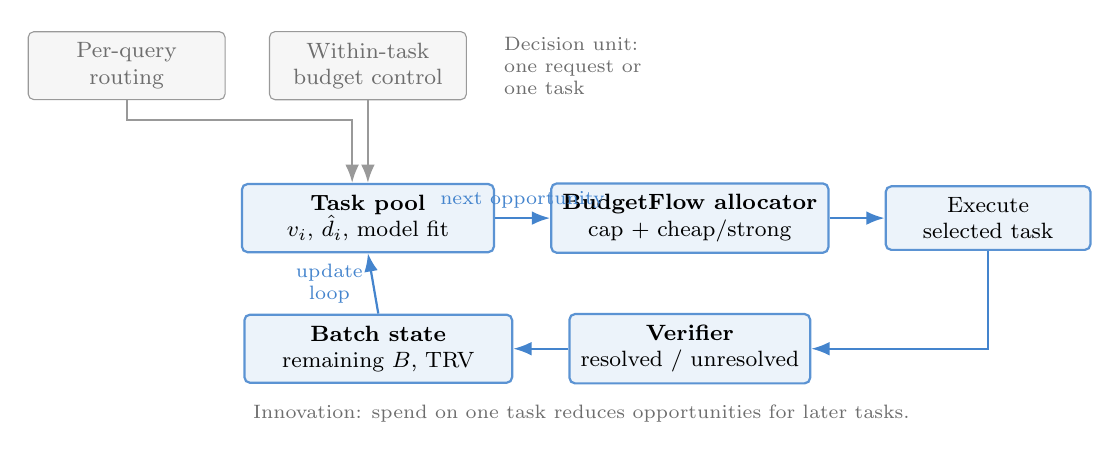
\begin{tikzpicture}[
  font=\footnotesize,
  >=Latex,
  box/.style={draw=bfblue!70, rounded corners=2pt, align=center, inner sep=4pt},
  main/.style={box, fill=bfblue!8, thick},
  soft/.style={box, draw=bfgray!70, fill=bfgray!6, text=bfgray},
  arrow/.style={->, thick, bfblue!80},
  softarrow/.style={->, thick, bfgray!70},
  note/.style={align=left, text=bfgray, font=\scriptsize}
]
\node[soft, minimum width=2.5cm] (q) {Per-query\\routing};
\node[soft, minimum width=2.5cm, right=0.55cm of q] (t) {Within-task\\budget control};
\node[note, right=0.35cm of t] (gap) {Decision unit:\\one request or\\one task};
\node[main, minimum width=3.2cm, below=1.05cm of t] (pool) {\textbf{Task pool}\\$v_i$, $\hat{d}_i$, model fit};
\node[main, minimum width=3.4cm, right=0.7cm of pool] (alloc) {\textbf{\method allocator}\\cap + cheap/strong};
\node[main, minimum width=2.6cm, right=0.7cm of alloc] (run) {Execute\\selected task};
\node[main, minimum width=2.8cm, below=0.75cm of alloc] (ver) {\textbf{Verifier}\\resolved / unresolved};
\node[main, minimum width=3.4cm, left=0.7cm of ver] (state) {\textbf{Batch state}\\remaining $B$, \trv};
\draw[softarrow] (q.south) -- ++(0,-0.25) -| ([xshift=-0.2cm]pool.north);
\draw[softarrow] (t.south) -- ++(0,-0.15) -- (pool.north);
\draw[arrow] (pool) -- node[above, font=\scriptsize]{next opportunity} (alloc);
\draw[arrow] (alloc) -- (run);
\draw[arrow] (run.south) |- (ver.east);
\draw[arrow] (ver) -- (state);
\draw[arrow] (state.north) -- node[left, font=\scriptsize, align=center]{update\\loop} (pool.south);
\node[note, below=0.15cm of state.south west, anchor=north west] {Innovation: spend on one task reduces opportunities for later tasks.};
\end{tikzpicture}
\caption{\method overview. Light boxes mark adjacent decision units. The main loop allocates across a task pool under one shared hard budget: choose the next task opportunity from frozen \taskvalue, estimated token cost, and model fit; execute; settle with a \verifier; update remaining budget and verified \trv.}
\label{fig:overview}
\end{figure*}

\section{Related Work}
\label{sec:related}
We organize related work by the decision problem it solves. Conference venues are not a ranking signal: newer papers are placed only by what decision they make.

\paragraph{Per-request cost--quality routing.}
RouteLLM learns per-query routers from preference data~\cite{routellm}. Cascade Routing studies model routing and cascading for individual queries~\cite{cascade-routing}. RouteNLP targets enterprise query routing under quality constraints~\cite{routenlp}. UCCI calibrates uncertainty for cost-optimal cascade routing~\cite{ucci}. ZeroRouter maps requests and models into a shared latent space for multi-objective routing and low-cost onboarding of new models~\cite{zerorouter}. Capability Instruction Tuning / MODEL-SAT selects models from capability instructions~\cite{model-sat}. ICL-Router and CP-Router further study request-level routing with in-context model representations or uncertainty-aware LLM/LRM choice~\cite{icl-router,cp-router}. These methods make model selection a first-class cost--quality problem for one prompt or one request. They do not allocate one shared hard budget across many tasks with unequal value.

\paragraph{Within-task budgeted agent control.}
INTENT plans costly tool use inside a single agent task under that task's own budget~\cite{intent}. BAMAS builds a multi-agent system for one task under a per-task cost cap by choosing models and collaboration structure~\cite{bamas}. Online Multi-LLM Selection adapts model choice over multi-turn interaction with a per-dialogue budget when the next prompt evolves as a black box~\cite{onlinemultillm}. CCPO orchestrates cheaper and stronger models inside one question under a reliability constraint~\cite{ccpo}. STEER switches between small and large models at reasoning steps using confidence signals~\cite{steer}. These methods optimize spend or model switches inside one task or one interaction. Even when a budget exists, it belongs to that task or dialogue, not to a batch of competing tasks.

\paragraph{Cost-aware agent runtimes.}
OpenSquilla is a token-efficient agent runtime with model routing, diagnostics, replay, and cost-per-success framing~\cite{opensquilla}. It strengthens the requirement that agent cost and execution behavior be measurable. Closely related harness-evaluation work such as Claw-SWE-Bench further stresses fair harness comparison and cost reporting~\cite{claw-swe-bench}, but it evaluates adapters rather than cross-task budget governance. \method uses a different decision unit: many tasks share one hard budget, and scarce strong-model opportunities should flow toward tasks that create the most verified value under frozen \taskvalue.

\section{Problem Formulation}
\label{sec:formulation}
Let a task batch contain tasks $\mathcal{T}=\{1,\ldots,n\}$ and let $B$ denote the \sharedbudget. Each task $i$ has a pre-registered value $v_i>0$, an estimated token cost $d_i>0$, and model-fit evidence $m_{i,k}$ for each model tier $k$. A policy $\pi$ chooses a sequence of actions that spend budget on model calls and task attempts. Let $c_i(\pi)$ be the spend on task $i$, and let
\[
    \sum_{i=1}^{n} c_i(\pi) \le B
\]
be the shared hard-budget constraint.

The budget is shared at the batch level. A policy can spend more on one task only by leaving less budget for later tasks in the same batch. This coupling is what separates the problem from independent per-task routing: a locally reasonable strong-model call can be globally poor if it consumes budget needed by a higher-value task.

Each task has a \verifier $V_i$ that maps the final task evidence to a binary outcome:
\[
    r_i(\pi)=V_i(\pi,i)\in\{0,1\}.
\]
The primary value objective is Total Resolved Value:
\[
    \mathrm{TRV}(\pi)=\sum_{i=1}^{n} v_i\,r_i(\pi).
\]
We report three headline metrics:
\[
    \mathrm{ResolvedRate}(\pi)=\frac{1}{n}\sum_{i=1}^{n}r_i(\pi),
\]
\[
    \mathrm{TRVperDollar}(\pi)=
    \frac{\mathrm{TRV}(\pi)}{\sum_i c_i(\pi)}.
\]

The \verifier settles outcomes after execution; allocation uses \taskvalue, \tokencost, \modelfit, and \sharedbudget state. In SWE-bench, $V_i$ is a test-based harness. \taskvalue is fixed before execution; \tokencost is a pre-run planning estimate; \modelfit can come from catalog priors or prior outcomes.

\section{BudgetFlow}
\label{sec:method}
\method maintains a \sharedbudget ledger across the task batch. For each task, it estimates whether the next model opportunity should use the cheap model, the strong model, or defer additional spend. The ledger is hard: \sharedbudget gates each planned action. The goal is to turn the general interface in Section~\ref{sec:formulation} into a concrete value-aware allocation policy.

The policy uses three allocation inputs:

\begin{itemize}
    \item $v_i$, the \taskvalue;
    \item $d_i$, the \tokencost;
    \item $m_{i,k}$, the \modelfit for tier $k$.
\end{itemize}

These inputs enter distinct decisions. \taskvalue prioritizes tasks that create more value if verified. \tokencost becomes cap planning: the policy estimates how much token cost a task may need before it can produce a useful artifact. \modelfit estimates whether the strong model is likely to improve the outcome relative to the cheap model. \sharedbudget controls affordability and stop/defer decisions.

Let $h$ denote budget pressure, with higher $h$ indicating tighter \sharedbudget state. Let $k_c$ be the cheap model and $k_s$ be the strong model. A simplified task-start score for giving task $i$ a strong-model opportunity is
\[
    S_i =
    \frac{v_i \cdot \max(m_{i,k_s}-m_{i,k_c},0)}
    {\max(d_i,\epsilon)}
    \cdot q(h),
\]
where $d_i$ is the task's \tokencost and $q(h)$ reduces strong-model access as \sharedbudget tightens. At task start, \method assigns a route and cap; during execution it can grant a strong-model opportunity or stop/defer when upside is low or the batch budget is threatened. Allocation and outcome settlement stay separate: the \verifier evaluates the final artifact after the attempt.

\begin{algorithm}[t]
\caption{BudgetFlow batch policy sketch}
\label{alg:budgetflow}
\begin{algorithmic}[1]
\STATE \textbf{Initialize} \sharedbudget state $R \leftarrow B$.
\FOR{task $i$ in the batch}
    \STATE \textbf{Read} $(v_i,d_i,m_{i,k_c},m_{i,k_s})$ and current $R$.
    \STATE \textbf{Set} an initial task cap from \taskvalue, \tokencost, and $R$.
    \STATE \textbf{Choose} cheap or strong model from \modelfit, value upside, and affordability.
    \STATE \textbf{Execute} the task while updating spend and \sharedbudget.
    \STATE \textbf{Continue}, \textbf{stop}, or \textbf{defer} using value upside and budget pressure.
    \STATE \textbf{Settle} the final artifact with $V_i$ and record $r_i$.
\ENDFOR
\STATE \textbf{Report} Resolved Rate, \trv, \trv per Dollar, and total spend.
\end{algorithmic}
\end{algorithm}

\section{Experimental Setup}
\label{sec:setup}
\paragraph{Task set.}
We evaluate on fixed 30-task SWE-bench-style bug-fixing batches. Each task requires an agent to inspect a repository, edit code, and produce a patch. Outcomes are scored by a local test-based harness, and every run exports official-format predictions for independent re-evaluation. Task values are pre-registered before execution.

\paragraph{Policies.}
Table~\ref{tab:policies} compares the five policies by the inputs they use. All policies run under the same shared hard budget and the same verifier. The key contrast is whether \taskvalue enters allocation of scarce model opportunities.

All policies share the same task order, budget protocol, model-tier catalog, and verifier. Batches differ in whether \tokencost/\modelfit use metadata-only estimates or prior-batch observations, and in the value ledger; hard caps are \$9.95 (5-policy) or \$10.44 stage-prefix pressure (4-policy).

\begin{table}[t]
\centering
\small
\begin{tabular}{lccc}
\toprule
Policy & Task Value & Model choice \\
\midrule
cheap-model-only &  & fixed cheap \\
strong-model-only &  & fixed strong \\
learned task-router &  & value-blind learned \\
budget-only &  & budget pressure \\
\textbf{\method} & yes & value-aware \\
\bottomrule
\end{tabular}
\caption{Policy inputs under the same shared hard budget and verifier.}
\label{tab:policies}
\end{table}

\paragraph{Metrics and sensitivity.}
We report Resolved Rate, \trv, and \trv per Dollar. Sensitivity replays one completed 5-policy batch under alternate value profiles or budget caps without new paid runs.

\section{Results}
\label{sec:results}
Table~\ref{tab:main-evidence} summarizes four paid 30-task batches. Red entries mark \method frontier signals; blue entries mark the strongest control in each group.

In the 4-policy BudgetFlow Pareto case, \method reaches \textbf{\trv 18.50 at \$7.98}, while strong-model-only reaches \trv 18.00 at \$9.46---higher value at about 16\% lower spend despite one fewer resolved task. In the 5-policy BudgetFlow leads-all case, \method resolves 16/30 tasks, reaches \trv 18.00, and achieves 1.81 \trv per Dollar, ahead of the learned task-router on all three metrics. The two Strong Coverage batches show broad strong-model use as the observed frontier, once with a larger lead and once with a close lead. Together, the evidence supports three frontier modes: \textbf{Value-Aware Budget Flow} (central \method target), \textbf{Strong Coverage} (strong model cost-effective under the cap), and \textbf{Model Fit} (accurate tier routing under extreme cache discounts; see sensitivity).

\begin{table*}[t]
\centering
\small
\begin{tabular}{@{}>{\raggedright\arraybackslash}p{0.28\textwidth}lcccc@{}}
\toprule
Batch reading & Policy & Resolved Rate & Spend & TRV & TRV per Dollar \\
\midrule
\textbf{BudgetFlow Pareto}: higher \trv at lower spend & \method & 14/30 (46.7\%) & \$7.98 & \pos{18.50} & \pos{2.32} \\
 & strong-model-only & \ctrl{15/30 (50.0\%)} & \$9.46 & 18.00 & 1.90 \\
\addlinespace
\textbf{Strong Coverage}: larger strong-model lead & strong-model-only & \ctrl{17/30 (56.7\%)} & \$9.95 & \ctrl{20.00} & \ctrl{2.01} \\
 & \method & 15/30 (50.0\%) & \$9.95 & 17.50 & 1.76 \\
\addlinespace
\textbf{Strong Coverage}: close strong-model lead & strong-model-only & \ctrl{18/30 (60.0\%)} & \$9.88 & \ctrl{19.00} & \ctrl{1.92} \\
 & \method & 17/30 (56.7\%) & \$9.95 & 18.50 & 1.86 \\
\addlinespace
\textbf{BudgetFlow leads all}: all primary metrics & \method & \pos{16/30 (53.3\%)} & \$9.95 & \pos{18.00} & \pos{1.81} \\
 & learned task-router & 15/30 (50.0\%) & \$9.95 & 17.00 & 1.71 \\
 & strong-model-only & 15/30 (50.0\%) & \$9.95 & 16.50 & 1.66 \\
\bottomrule
\end{tabular}
\caption{Main paid evidence. Each group is one 30-task batch. Red bold: \method frontier signals; blue bold: strongest control.}
\label{tab:main-evidence}
\end{table*}

\section{Sensitivity Analysis}
\label{sec:sensitivity}
Sensitivity replays fixed outcomes from the 5-policy BudgetFlow leads-all case. Table~\ref{tab:value-sensitivity} re-scores under alternate Task Value profiles; \method stays ahead with median margin +1.00 \trv over 64 permutations. Budget replay at sampled caps moves the batch between Strong Coverage and Value-Aware Budget Flow; under extreme KV-cache discounts, learned routing briefly leads on \trv per Dollar while \method keeps higher \trv.

\begin{table}[t]
\centering
\small
\begin{tabular}{lccc}
\toprule
Value profile & BF TRV & Control TRV & Margin \\
\midrule
equal & \pos{16.00} & 15.00 & \pos{+1.00} \\
criticality & \pos{18.00} & 17.00 & \pos{+1.00} \\
compressed & \pos{17.00} & 16.00 & \pos{+1.00} \\
expanded & \pos{20.00} & 19.00 & \pos{+1.00} \\
\bottomrule
\end{tabular}
\caption{Task Value sensitivity on the 5-policy case.}
\label{tab:value-sensitivity}
\end{table}

\section{Discussion and Conclusion}
\label{sec:discussion}
The SWE-bench experiments instantiate a domain-neutral contract: tasks expose \taskvalue, \tokencost, \modelfit, and a \verifier under one \sharedbudget. Frontier-mode reporting makes mixed outcomes interpretable---Strong Coverage when the strong model is broadly cost-effective, Model Fit when tier routing dominates under serving discounts, and Value-Aware Budget Flow when unequal task value forces cross-task tradeoffs. Future work can add finer within-task control, auditable learning from completed batches, and serving-aware multi-tenant scheduling above inference substrates.

\method formulates Batch-Level Task Budget Allocation and separates allocation signals from \verifier-settled outcomes. On SWE-bench, it improves the spend--\trv frontier in one batch and leads Resolved Rate, \trv, and \trv per Dollar in another under the same hard cap. The transferable object is the interface for governing verified value under fixed resource constraints.


\bibliography{references}
\end{document}
